\setcounter{chapter}{5}
\chapter{Faz Düzlemi}

\section{Faz Portreleri}

\begin{justify}
Faz düzlemindeki bir vektör alanının genel biçimi
\begin{align}
\dot{x}_1 &= f_1(x_1,x_2),\\
\dot{x}_2 &= f_2(x_1,x_2),
\end{align}
şeklindedir. Burada $f_1$ ve $f_2$ verilen fonksiyonlardır. Bu sistem, vektör gösterimiyle daha kısa biçimde
\begin{equation}
\dot{\mathbf{x}}=\mathbf{f}(\mathbf{x})
\end{equation}
olarak yazılabilir. Burada $\mathbf{x}=(x_1,x_2)$ ve $\mathbf{f}(\mathbf{x})=(f_1(\mathbf{x}),f_2(\mathbf{x}))$ olur. $\mathbf{x}$ faz düzlemindeki bir noktayı, $\dot{\mathbf{x}}$ ise bu noktadaki hız vektörünü temsil eder. Vektör alanı boyunca hareket eden bir faz noktası, faz düzleminde ilerleyen bir yörüngeye karşılık gelen $\mathbf{x}(t)$ çözümünü çizer (Şekil~\ref{fig:6-1-1}). Ayrıca faz düzleminin tamamı yörüngelerle doludur; çünkü her nokta bir başlangıç koşulu olarak alınabilir.

\begin{figure}[H]
\centering
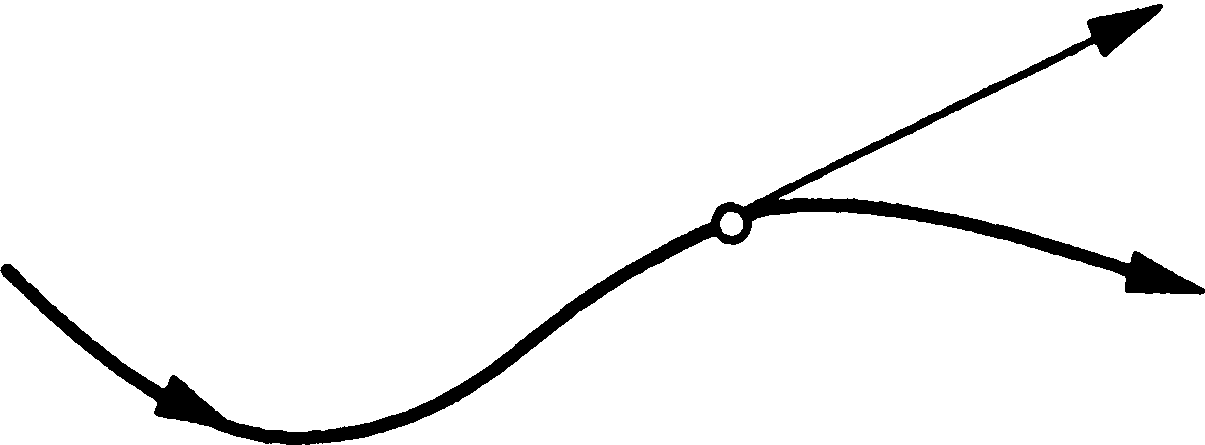
\includegraphics[width=0.82\textwidth]{images/Figures/figur-002.png}
\caption{Faz düzleminde bir yörüngenin gösterimi.}
\label{fig:6-1-1}
\end{figure}

Doğrusal olmayan sistemlerde yörüngeleri analitik olarak bulmak çoğu zaman mümkün değildir. Açık formüller elde edilebildiği durumlarda bile bu formüller genellikle anlamlı bir kavrayış sağlayamayacak kadar karmaşık olur. Bu nedenle çözümlerin nitel davranışını belirlemeye çalışacağız. Amacımız, sistemin faz portresini doğrudan $\mathbf{f}(\mathbf{x})$ fonksiyonunun özelliklerinden çıkarmaktır. Çok çeşitli faz portreleri ortaya çıkabilir; bunun bir örneği Şekil~\ref{fig:6-1-2}'de gösterilecektir.

\begin{figure}[H]
\centering
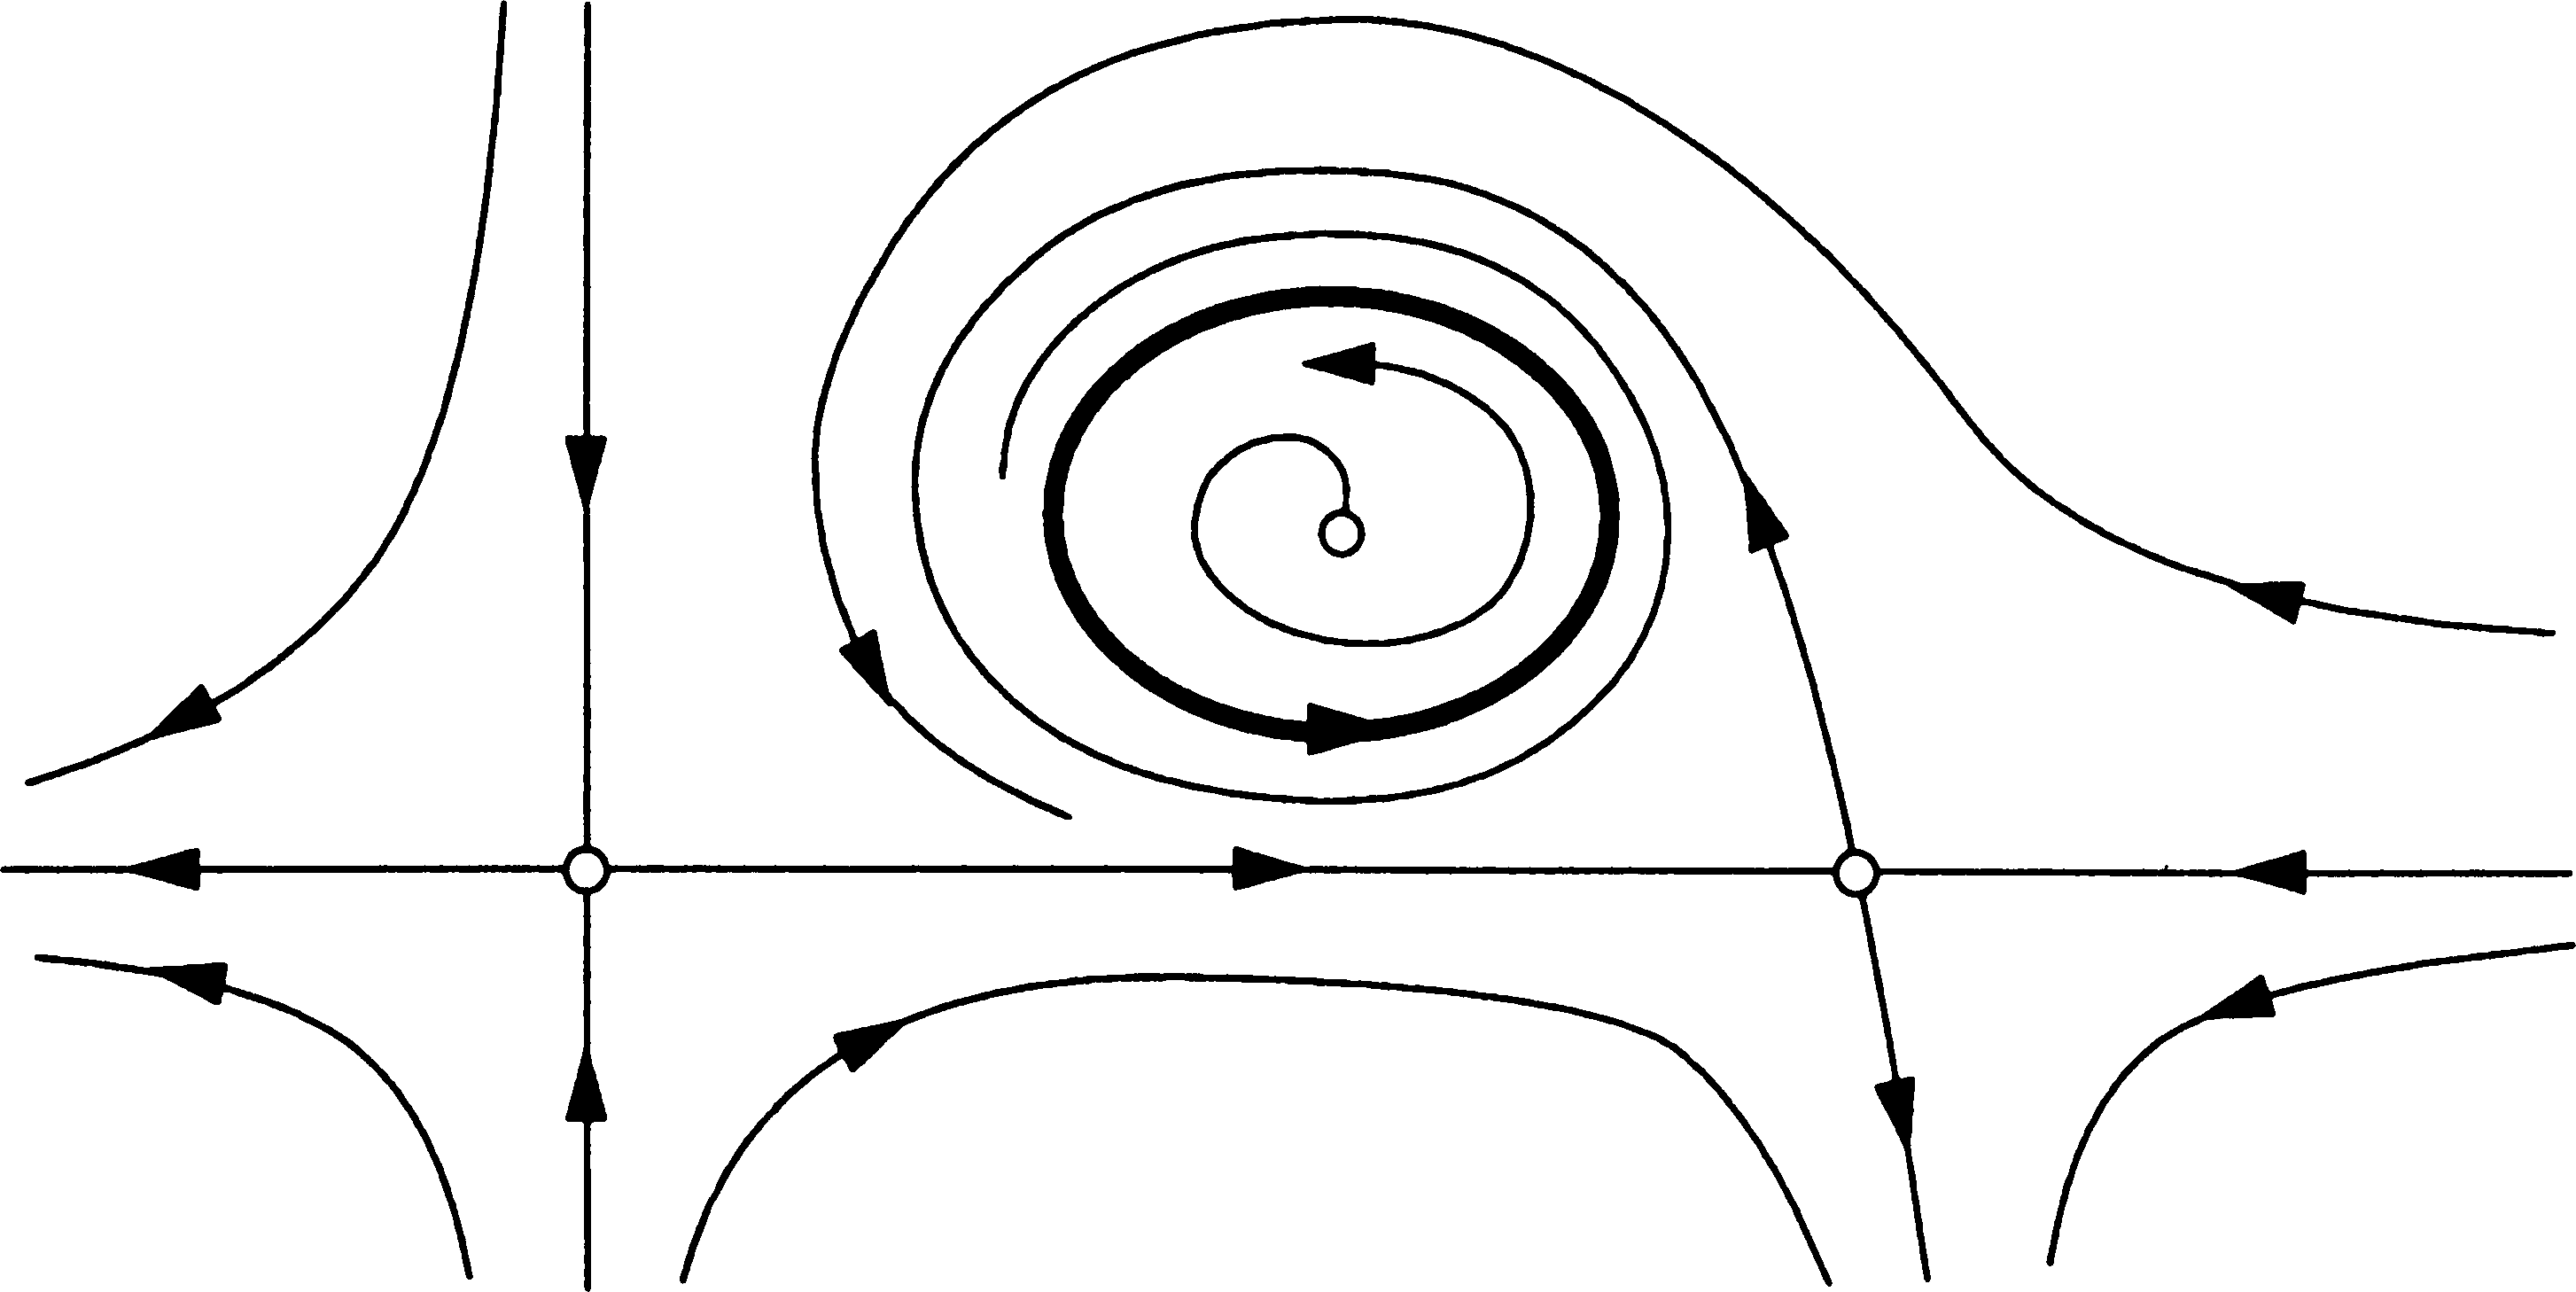
\includegraphics[width=0.82\textwidth]{images/Figures/figur-001.png}
\caption{Sabit noktalar ve kapalı yörünge içeren örnek faz portresi.}
\label{fig:6-1-2}
\end{figure}

Herhangi bir faz portresinin en belirgin özelliklerinden bazıları şunlardır:
\begin{enumerate}
\item \textbf{Sabit noktalar:} Şekil~\ref{fig:6-1-2}'deki $A$, $B$ ve $C$ gibi noktalar sabit noktalardır. Sabit noktalar $\mathbf{f}(\mathbf{x}^{*})=0$ koşulunu sağlar ve sistemin kararlı durumlarına ya da dengelerine karşılık gelir.
\item \textbf{Kapalı yörüngeler:} Şekil~\ref{fig:6-1-2}'deki $D$ gibi kapalı eğriler periyodik çözümleri temsil eder. Başka bir deyişle, bir $T>0$ değeri için tüm $t$ değerlerinde
\begin{equation}
\mathbf{x}(t+T)=\mathbf{x}(t)
\end{equation}
koşulu sağlanır.
\item \textbf{Yörüngelerin yerleşimi:} Sabit noktaların ve kapalı yörüngelerin yakınındaki yörünge düzeni önemlidir. Örneğin $A$ ve $C$ yakınındaki akış deseni birbirine benzerken, $B$ yakınındaki desenden farklıdır.
\item \textbf{Kararlılık ya da kararsızlık:} Sabit noktaların ve kapalı yörüngelerin kararlı olup olmadığı faz portresinin temel özelliklerindendir. Örneğin $A$, $B$ ve $C$ sabit noktaları kararsızdır; çünkü yakınlarındaki yörüngeler bu noktalardan uzaklaşma eğilimindedir. Buna karşılık $D$ kapalı yörüngesi kararlıdır.
\end{enumerate}
\end{justify}

\subsection*{Faz Portrelerinin Sayısal Hesaplanması}
\phantomsection
\addcontentsline{toc}{subsection}{Faz Portrelerinin Sayısal Hesaplanması}

\begin{justify}
Bazı durumlarda faz portresinin nicel özellikleriyle de ilgileniriz. Neyse ki $\dot{\mathbf{x}}=\mathbf{f}(\mathbf{x})$ sisteminin sayısal integrasyonu, tek değişkenli $\dot{x}=f(x)$ denkleminin sayısal integrasyonundan çok daha zor değildir. Önceki sayısal yöntemler, $x$ ve $f(x)$ sayıları yerine $\mathbf{x}$ ve $\mathbf{f}(\mathbf{x})$ vektörleri kullanıldığında yine geçerlidir.

Bu çalışmada Runge--Kutta yöntemi kullanılacaktır. Yöntemin vektörel biçimi
\begin{equation}
\mathbf{x}_{n+1}=\mathbf{x}_n+\frac{1}{6}\left(\mathbf{k}_1+2\mathbf{k}_2+2\mathbf{k}_3+\mathbf{k}_4\right)
\end{equation}
şeklindedir. Burada
\begin{align}
\mathbf{k}_1 &= \Delta t\,\mathbf{f}(\mathbf{x}_n),\\
\mathbf{k}_2 &= \Delta t\,\mathbf{f}\left(\mathbf{x}_n+\frac{1}{2}\mathbf{k}_1\right),\\
\mathbf{k}_3 &= \Delta t\,\mathbf{f}\left(\mathbf{x}_n+\frac{1}{2}\mathbf{k}_2\right),\\
\mathbf{k}_4 &= \Delta t\,\mathbf{f}\left(\mathbf{x}_n+\mathbf{k}_3\right).
\end{align}
Amaçlarımız için genellikle $\Delta t=0.1$ adım büyüklüğü yeterli doğruluk sağlar.

Faz portresi çizilirken vektör alanındaki temsilî vektörlerden oluşan bir ızgarayı görmek çoğu zaman yararlıdır. Ancak ok uçları ve vektör uzunluklarının farklı olması bu tür çizimleri kalabalıklaştırabilir. Bu nedenle yön alanı çizimi daha açık bir görünüm sağlar: Akışın yerel yönünü göstermek için kısa doğru parçaları kullanılır.
\end{justify}

\subsection*{Örnek 6.1.1}
\phantomsection
\addcontentsline{toc}{subsection}{Örnek 6.1.1}

\begin{justify}
Aşağıdaki sistemi ele alalım:
\begin{align}
\dot{x} &= x+e^{-y},\\
\dot{y} &= -y.
\end{align}
Önce nitel argümanlar kullanarak faz portresi hakkında bilgi elde edelim. Daha sonra bilgisayar yardımıyla yön alanını çizelim. Son olarak Runge--Kutta yöntemini kullanarak birkaç yörünge hesaplayalım ve bunları faz düzleminde gösterelim.

\textbf{Çözüm.} İlk olarak sabit noktaları bulmak için $\dot{x}=0$ ve $\dot{y}=0$ denklemlerini birlikte çözeriz. Tek çözüm
\begin{equation}
(x^{*},y^{*})=(-1,0)
\end{equation}
olarak bulunur.

Bu sabit noktanın kararlılığını belirlemek için $y(t)$ davranışına bakalım. $\dot{y}=-y$ denkleminin çözümü
\begin{equation}
y(t)=y_0e^{-t}
\end{equation}
olduğundan $t\to\infty$ iken $y(t)\to 0$ olur. Dolayısıyla uzun vadede $e^{-y}\to 1$ ve $x$ için denklem yaklaşık olarak
\begin{equation}
\dot{x}=x+1
\end{equation}
haline gelir. Bu denklem üstel olarak büyüyen çözümlere sahiptir; bu da sabit noktanın kararsız olduğunu düşündürür. Gerçekte, başlangıç koşullarını $x$ ekseni üzerinde seçersek $y_0=0$ olur ve bundan dolayı tüm zamanlar için $y(t)=0$ kalır. Bu durumda $x$ ekseni üzerindeki akış tamamen $\dot{x}=x+1$ denklemi tarafından belirlenir. Bu nedenle sabit nokta kararsızdır.

Faz portresini çizmek için nulklinleri belirlemek yararlıdır. Nulklinler, $\dot{x}=0$ ya da $\dot{y}=0$ koşullarından birinin sağlandığı eğrilerdir. Bu eğriler akışın nerede tamamen yatay veya tamamen düşey olduğunu gösterir (Şekil~\ref{fig:6-1-3}).

Örneğin akış $\dot{y}=0$ olduğu yerlerde yataydır. $\dot{y}=-y$ olduğundan bu durum $y=0$ doğrusu üzerinde gerçekleşir. Bu doğru boyunca $\dot{x}=x+1$ olur. Dolayısıyla $x>-1$ iken akış sağa doğrudur.

Benzer şekilde akış $\dot{x}=x+e^{-y}=0$ olduğu yerlerde düşeydir. Bu koşul
\begin{equation}
x=-e^{-y}
\end{equation}
eğrisini verir. Eğrinin $y>0$ olan üst kısmında akış aşağı yönlüdür; çünkü burada $\dot{y}<0$ olur.

Nulklinler ayrıca düzlemi, $\dot{x}$ ve $\dot{y}$ işaretlerinin farklı değerler aldığı bölgelere ayırır. Şekil~\ref{fig:6-1-3}'te bu bölgelerdeki tipik vektör yönleri gösterilecektir. Bu bilgiler tek başına bile genel akış deseninin anlaşılması için iyi bir başlangıç sağlar.

\begin{figure}[H]
\centering
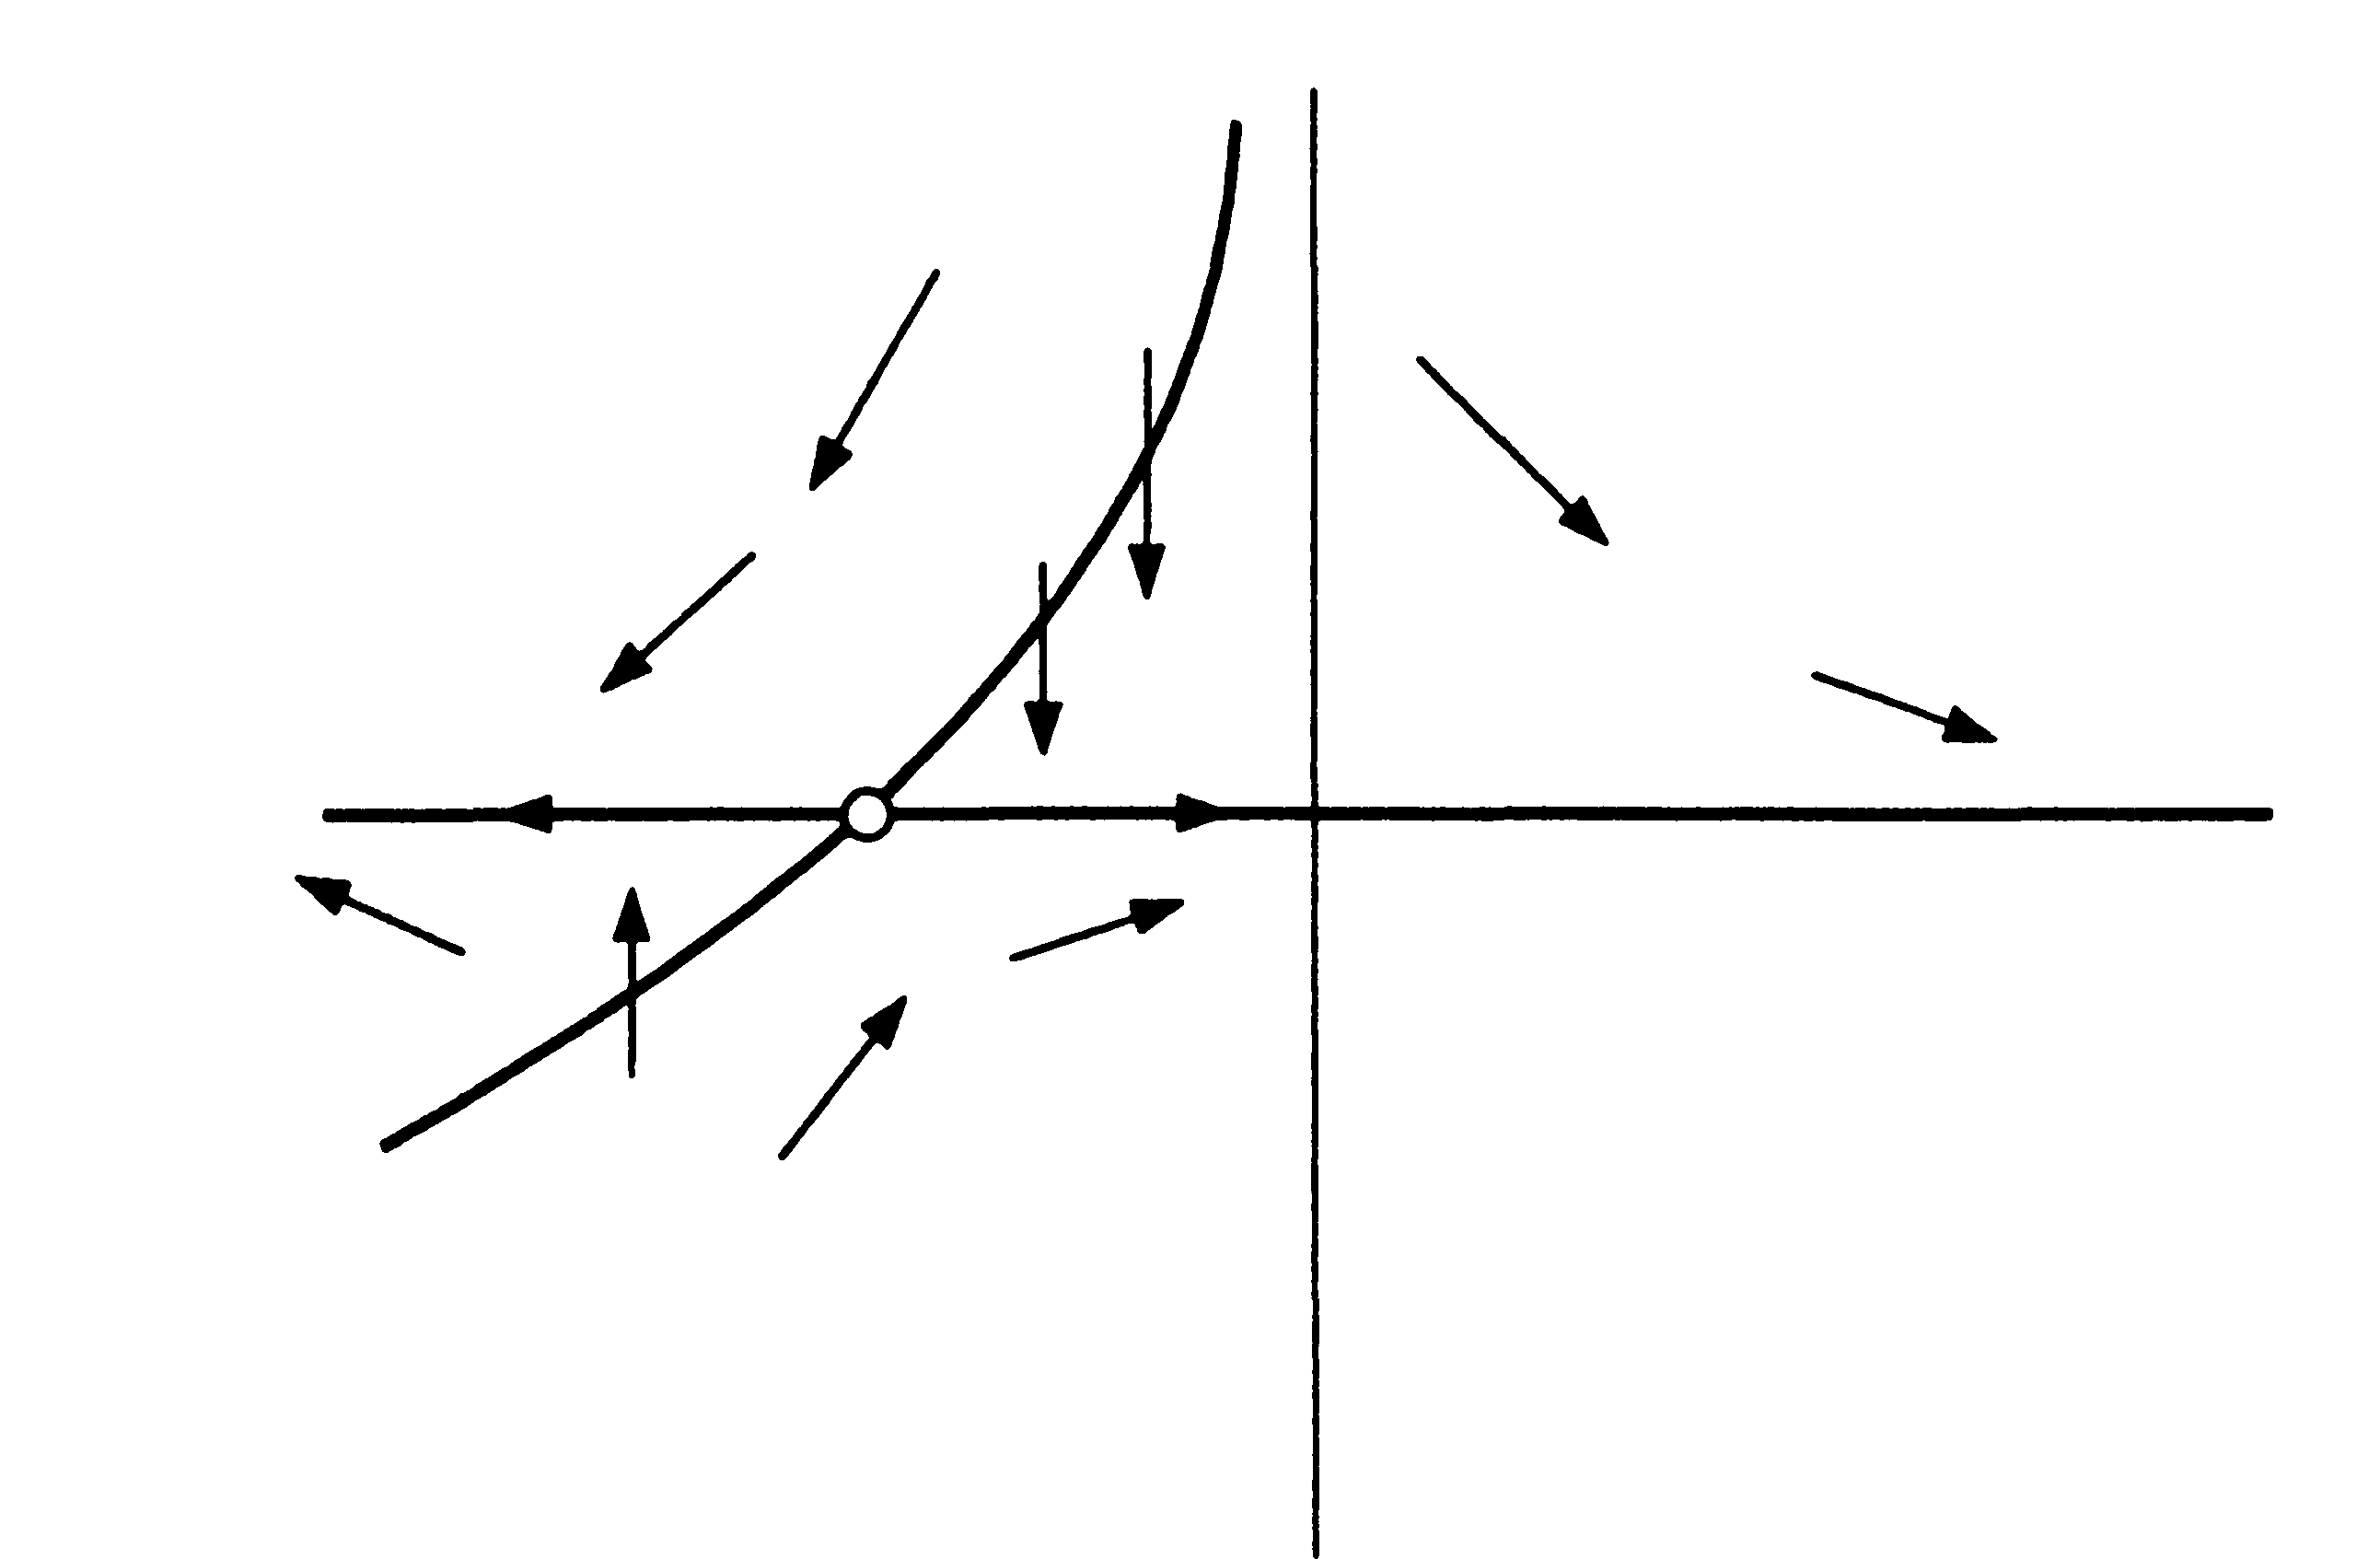
\includegraphics[width=0.82\textwidth]{images/Figures/figur-003.png}
\caption{Örnek 6.1.1 için nulklinler ve bölgelerdeki akış yönleri.}
\label{fig:6-1-3}
\end{figure}

Şimdi problemi tamamlamak için bilgisayar kullanılır. Şekil~\ref{fig:6-1-4}'te yön alanı kısa doğru parçalarıyla gösterilecek ve birkaç yörünge çizilecektir. Yörüngelerin her noktada yerel eğimi izlediği görülür. Böylece sabit noktanın, doğrusal olmayan bir eyer noktası türü olduğu anlaşılır.

\begin{figure}[H]
\centering
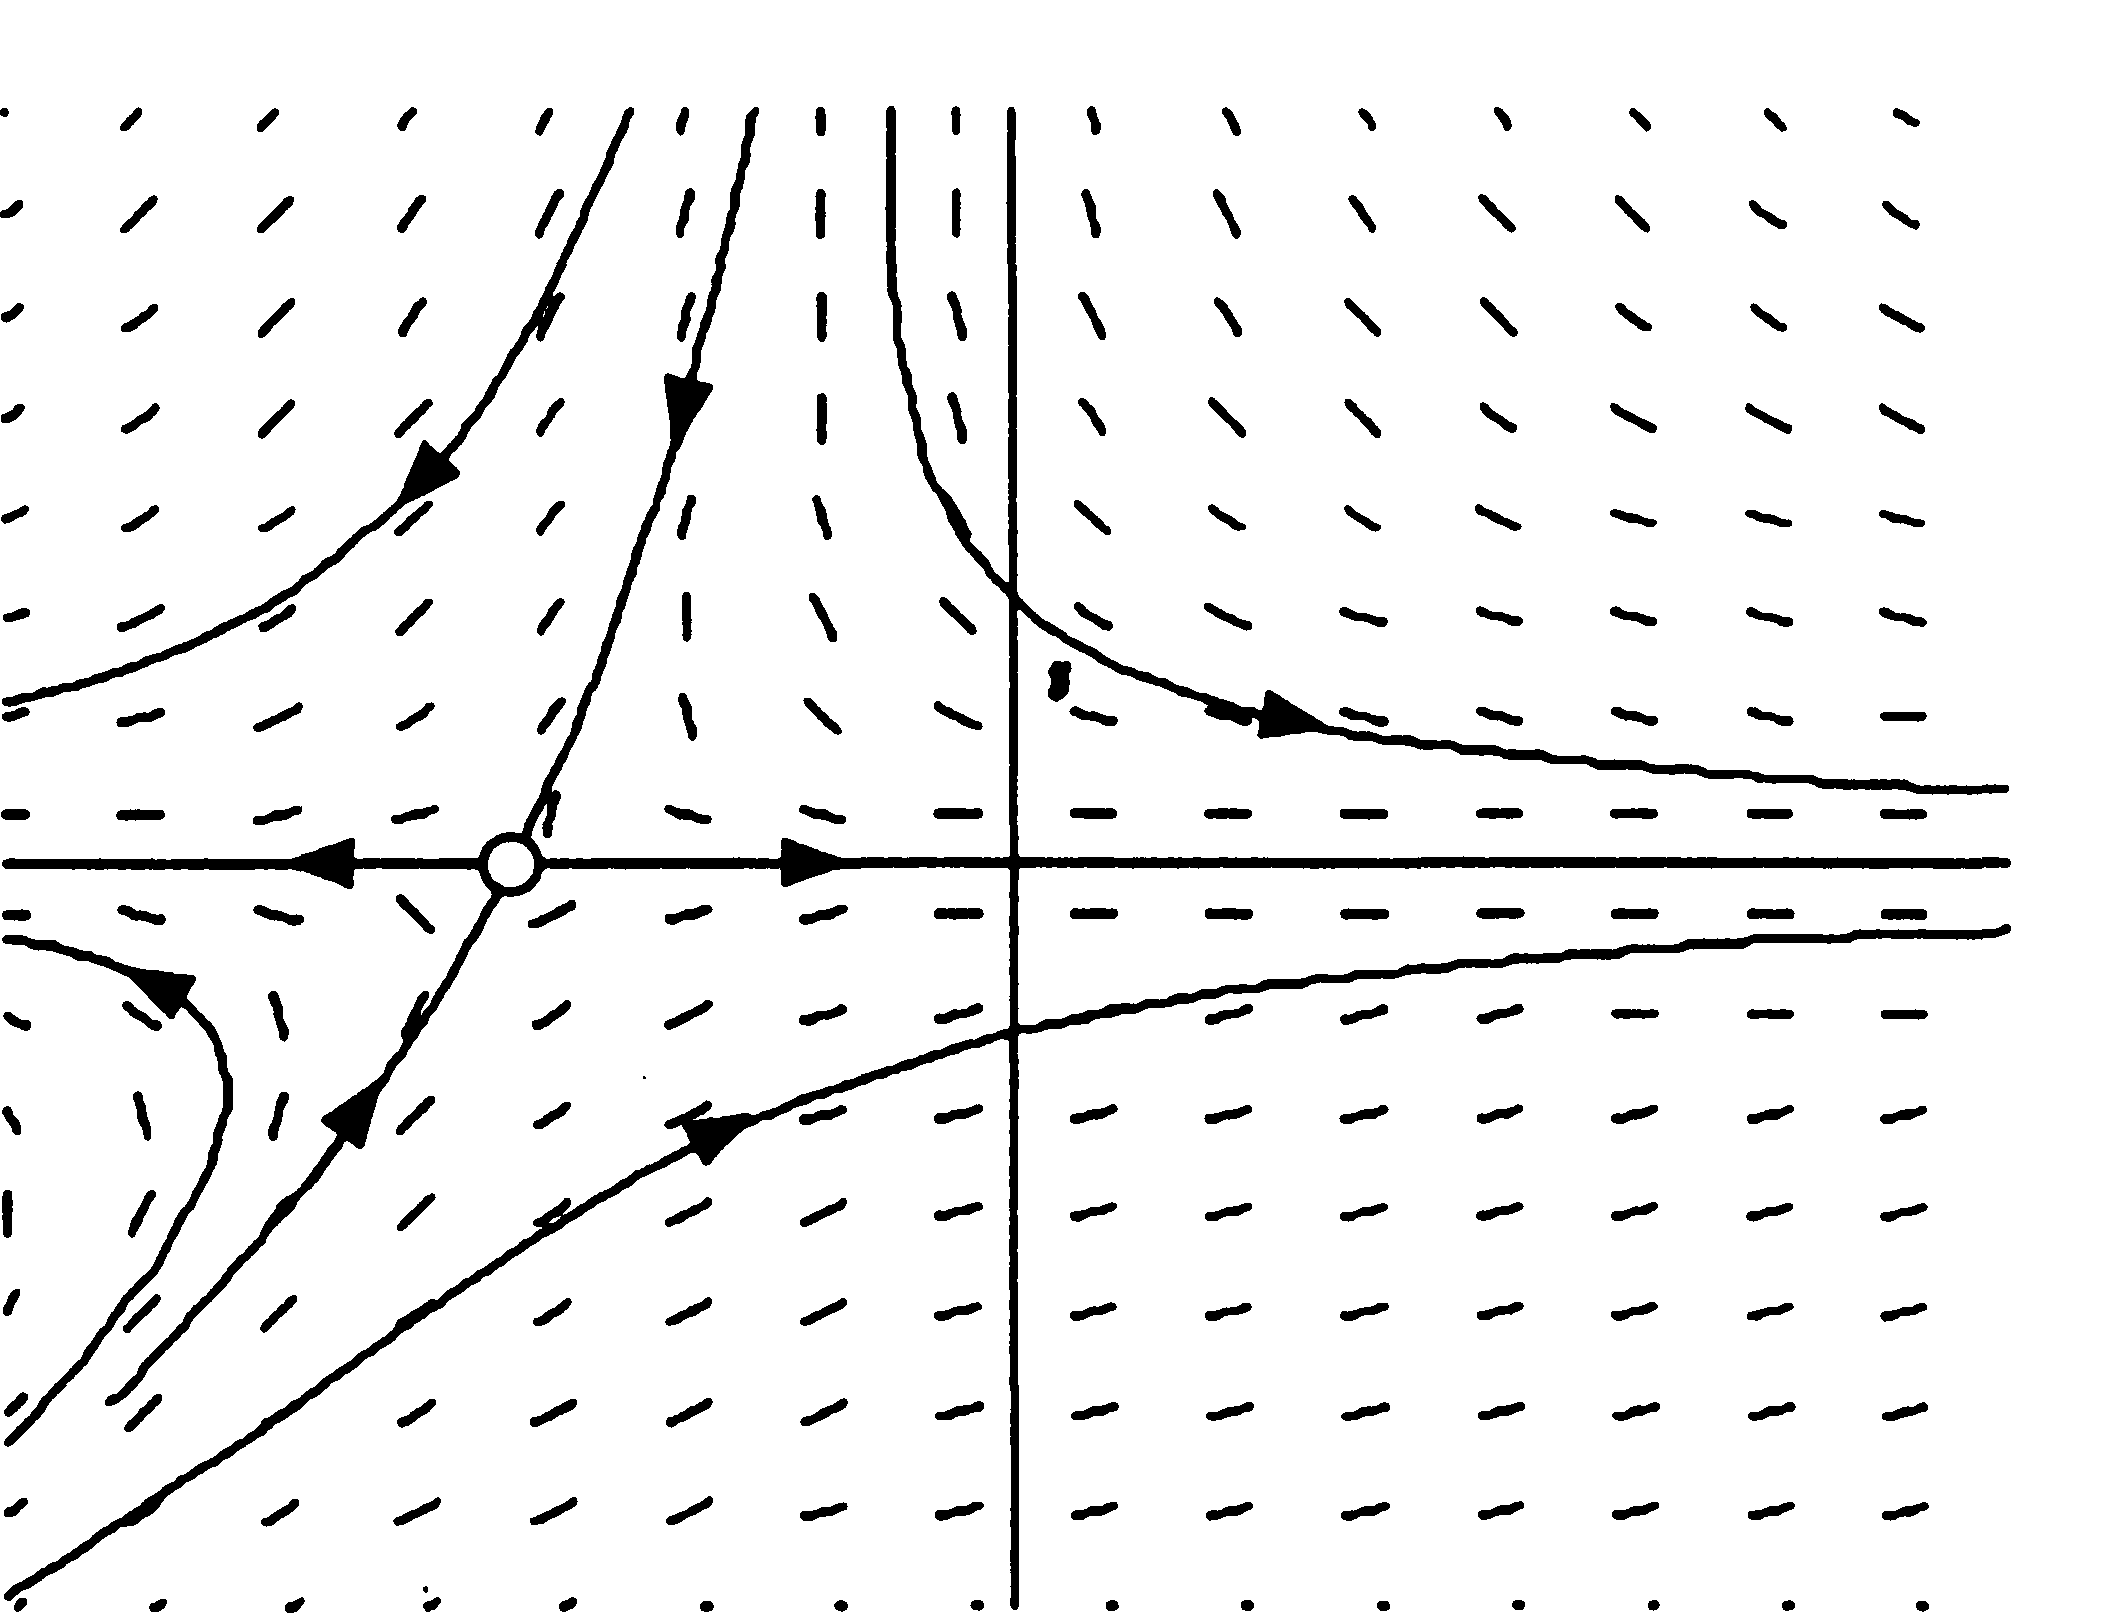
\includegraphics[width=0.82\textwidth]{images/Figures/figur-004.png}
\caption{Örnek 6.1.1 için yön alanı ve seçilmiş yörüngeler.}
\label{fig:6-1-4}
\end{figure}
\end{justify}

\section{Varlık, Teklik ve Topolojik Sonuçlar}

\begin{justify}
Şimdiye kadar biraz iyimser davrandık; bu aşamada genel doğrusal olmayan sistem
\begin{equation}
\dot{\mathbf{x}}=\mathbf{f}(\mathbf{x})
\end{equation}
için çözümlerin var olduğuna dair henüz bir güvencemiz yoktur. Neyse ki Bölüm 2.5'te verilen varlık ve teklik teoremi iki boyutlu sistemlere genelleştirilebilir. Ek bir zorluk içermediği için sonuç $n$ boyutlu sistemler için ifade edilir.

\textbf{Varlık ve Teklik Teoremi.} Başlangıç değer problemini ele alalım:
\begin{equation}
\dot{\mathbf{x}}=\mathbf{f}(\mathbf{x}), \qquad \mathbf{x}(0)=\mathbf{x}_0.
\end{equation}
$\mathbf{f}$ sürekli olsun ve tüm kısmi türevleri
\begin{equation}
\frac{\partial f_i}{\partial x_j}, \qquad i,j=1,\ldots,n,
\end{equation}
$D\subset \mathbb{R}^n$ olan açık ve bağlantılı bir kümede sürekli olsun. O hâlde $\mathbf{x}_0\in D$ için başlangıç değer probleminin $t=0$ etrafındaki bir $(-\tau,\tau)$ zaman aralığında bir çözümü vardır ve bu çözüm tektir.

Başka bir deyişle, $\mathbf{f}$ sürekli türevlenebilirse çözümlerin varlığı ve tekliği güvence altındadır. Teoremin ispatı $n=1$ durumu için yapılan ispata benzerdir ve diferansiyel denklemler üzerine yazılmış çoğu kaynakta bulunabilir. Teoremin daha güçlü biçimleri de vardır; ancak bu biçim çoğu uygulama için yeterlidir.

Bundan sonra, ele alınan tüm vektör alanlarının faz uzayındaki herhangi bir noktadan başlayan çözümlerin varlığını ve tekliğini sağlayacak kadar düzgün olduğunu kabul edeceğiz.

Varlık ve teklik teoreminin önemli bir sonucu vardır: farklı yörüngeler asla kesişmez. Eğer iki yörünge kesişseydi, aynı noktadan, yani kesişim noktasından başlayan iki farklı çözüm olurdu. Bu durum teoremin teklik kısmıyla çelişirdi. Daha sezgisel bir ifadeyle, bir yörünge aynı anda iki farklı yönde hareket edemez.

Yörüngeler kesişemediği için faz portreleri her zaman düzenli bir görünüme sahiptir. Aksi hâlde, birbirini kesen eğrilerden oluşan karmaşık bir düğüme dönüşebilirlerdi (Şekil~\ref{fig:6-2-1}). Varlık ve teklik teoremi bunun olmasını engeller.

\begin{figure}[H]
\centering
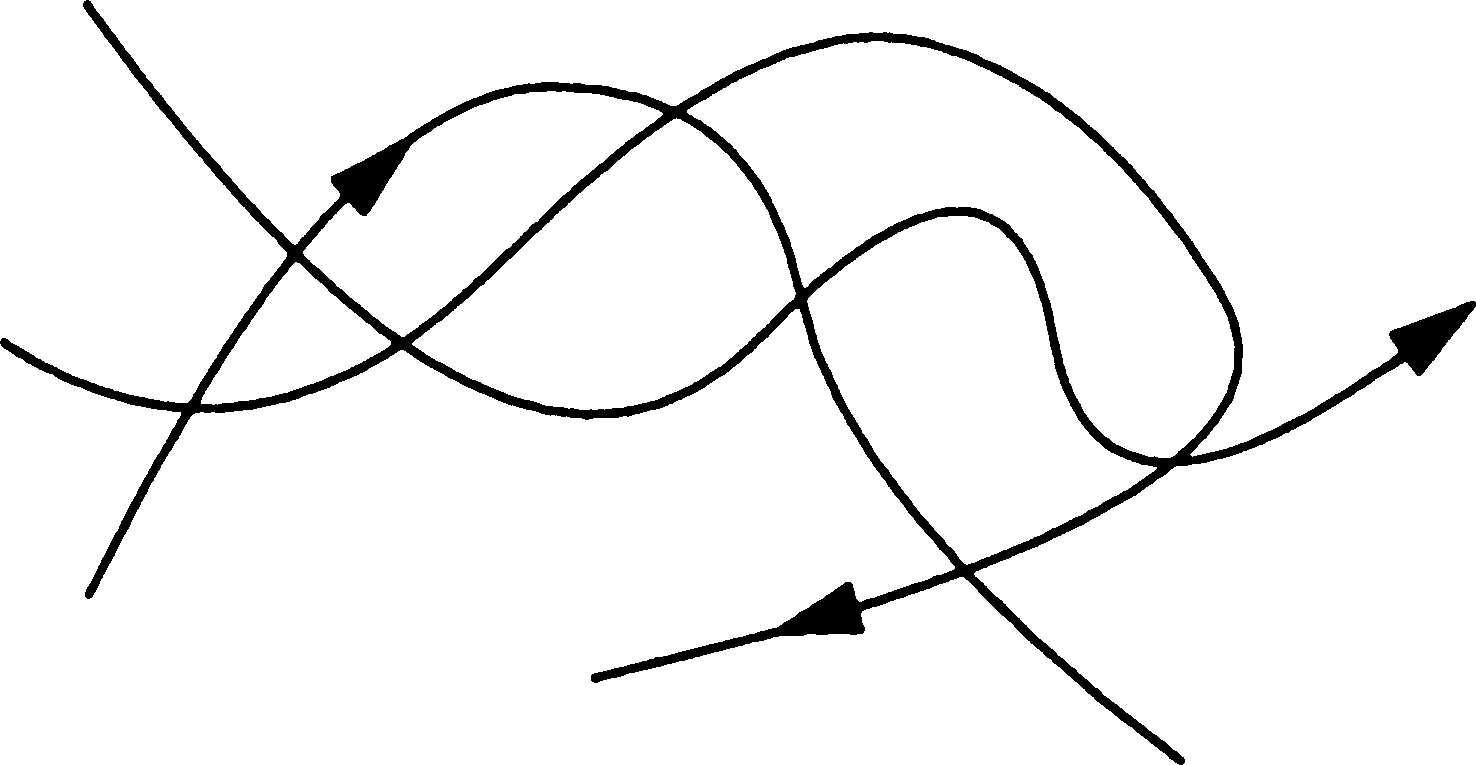
\includegraphics[width=0.82\textwidth]{images/Figures/figur-005.png}
\caption{Teklik özelliği olmasaydı ortaya çıkabilecek, birbirini kesen yörüngelerden oluşan düzensiz görünüm.}
\label{fig:6-2-1}
\end{figure}

İki boyutlu faz uzaylarında, daha yüksek boyutlu faz uzaylarından farklı olarak, bu sonuçların özellikle güçlü topolojik sonuçları vardır. Örneğin faz düzleminde kapalı bir $C$ yörüngesi bulunduğunu varsayalım. Bu durumda $C$ içinde başlayan herhangi bir yörünge sonsuza kadar bu bölgenin içinde hapsolur (Şekil~\ref{fig:6-2-2}).

\begin{figure}[H]
\centering
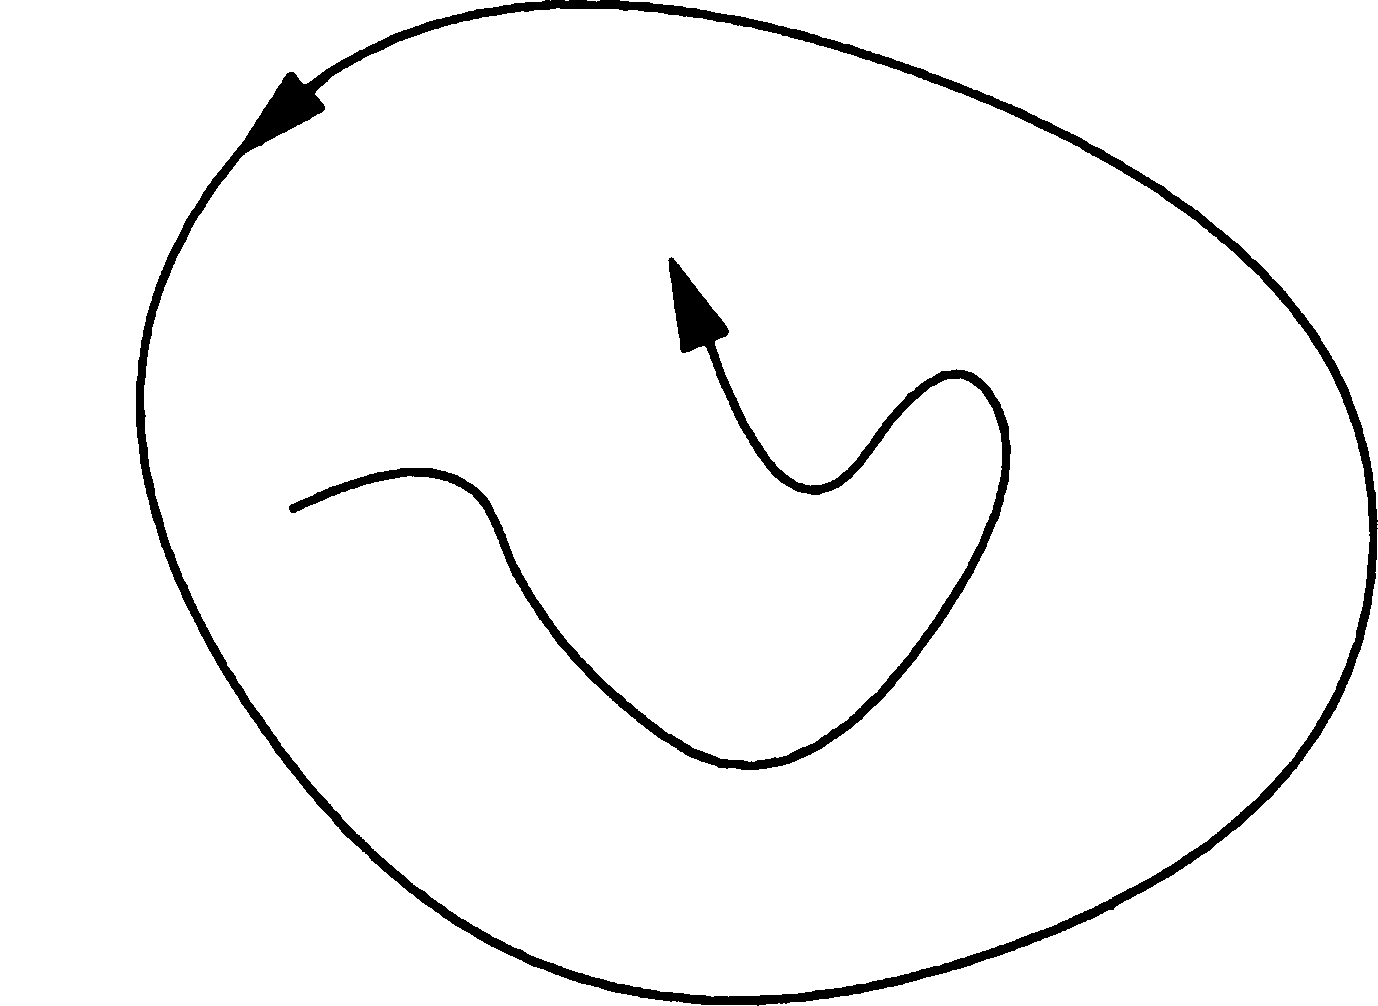
\includegraphics[width=0.82\textwidth]{images/Figures/figur-006.png}
\caption{Kapalı bir yörünge içinde başlayan yörüngenin içeride hapsolması.}
\label{fig:6-2-2}
\end{figure}

Peki böyle sınırlı bir yörüngenin sonu ne olur? Eğer $C$ içinde sabit noktalar varsa, yörünge elbette sonunda bunlardan birine yaklaşabilir. Fakat içeride hiç sabit nokta yoksa ne olur? Sezgileriniz yörüngenin sonsuza kadar gelişigüzel dolaşamayacağını söylüyorsa haklısınız. Düzlem üzerindeki vektör alanları için Poincaré--Bendixson teoremi şunu söyler: Bir yörünge kapalı ve sınırlı bir bölgede kalıyorsa ve bölgede sabit nokta yoksa, yörünge sonunda bir kapalı yörüngeye yaklaşmak zorundadır. Bu önemli teorem Bölüm 7.3'te tartışılacaktır.

Ancak hikâyenin bu kısmı daha sonra gelecektir. Önce sabit noktaları daha iyi tanımamız gerekir.
\end{justify}

\section{Sabit Noktalar ve Lineerleştirme}

\begin{justify}
Bu bölümde, daha önce tek boyutlu sistemler için geliştirilen lineerleştirme tekniğini genişletiyoruz. Umut edilen şey, bir sabit nokta yakınındaki faz portresinin, ona karşılık gelen doğrusal bir sistemin faz portresiyle yaklaşık olarak temsil edilebilmesidir.
\end{justify}

\subsection*{Lineerleştirilmiş Sistem}
\phantomsection
\addcontentsline{toc}{subsection}{Lineerleştirilmiş Sistem}

\begin{justify}
Aşağıdaki sistemi ele alalım:
\begin{align}
\dot{x} &= f(x,y),\\
\dot{y} &= g(x,y),
\end{align}
ve $(x^{*},y^{*})$ noktasının bir sabit nokta olduğunu varsayalım; yani
\begin{equation}
f(x^{*},y^{*})=0, \qquad g(x^{*},y^{*})=0.
\end{equation}
Sabit noktadan küçük bir sapmanın bileşenlerini
\begin{equation}
u=x-x^{*}, \qquad v=y-y^{*}
\end{equation}
ile gösterelim. Bu sapmanın büyüyüp büyümediğini ya da sönümlenip sönümlenmediğini görmek için $u$ ve $v$ için diferansiyel denklemler türetmemiz gerekir. Önce $u$ denklemini yazalım:
\begin{align}
\dot{u} &= \dot{x} && \text{çünkü } x^{*}\text{ sabittir},\\
&= f(x^{*}+u,y^{*}+v) && \text{yerine koyma ile},\\
&= f(x^{*},y^{*})+u\frac{\partial f}{\partial x}+v\frac{\partial f}{\partial y}+O(u^2,v^2,uv) && \text{Taylor açılımı ile},\\
&= u\frac{\partial f}{\partial x}+v\frac{\partial f}{\partial y}+O(u^2,v^2,uv) && \text{çünkü } f(x^{*},y^{*})=0.
\end{align}
Gösterimi sadeleştirmek için $\partial f/\partial x$ ve $\partial f/\partial y$ yazılmıştır; fakat bu kısmi türevlerin sabit nokta $(x^{*},y^{*})$ üzerinde değerlendirildiği unutulmamalıdır. Dolayısıyla bunlar fonksiyon değil, sayıdır. Ayrıca $O(u^2,v^2,uv)$ kısa gösterimi, $u$ ve $v$ cinsinden ikinci dereceden terimleri belirtir. $u$ ve $v$ küçük olduğundan, bu ikinci dereceden terimler son derece küçüktür.

Benzer şekilde
\begin{equation}
\dot{v}=u\frac{\partial g}{\partial x}+v\frac{\partial g}{\partial y}+O(u^2,v^2,uv)
\end{equation}
bulunur. Böylece $(u,v)$ sapması
\begin{equation}
\begin{pmatrix}\dot{u}\\ \dot{v}\end{pmatrix}
=
\begin{pmatrix}
\dfrac{\partial f}{\partial x} & \dfrac{\partial f}{\partial y}\\[0.3cm]
\dfrac{\partial g}{\partial x} & \dfrac{\partial g}{\partial y}
\end{pmatrix}
\begin{pmatrix}u\\ v\end{pmatrix}
+ \text{ikinci dereceden terimler}
\end{equation}
biçiminde evrilir. Buradaki
\begin{equation}
A=\begin{pmatrix}
\dfrac{\partial f}{\partial x} & \dfrac{\partial f}{\partial y}\\[0.3cm]
\dfrac{\partial g}{\partial x} & \dfrac{\partial g}{\partial y}
\end{pmatrix}_{(x^{*},y^{*})}
\end{equation}
matrisine sabit nokta $(x^{*},y^{*})$ üzerindeki Jacobian matrisi denir. Bu matris, Bölüm 2.4'te görülen $f'(x^{*})$ türevinin çok değişkenli karşılığıdır.

İkinci dereceden terimler çok küçük olduğundan, bunları tamamen ihmal etmek cazip görünür. Bunu yaptığımızda lineerleştirilmiş sistem elde edilir:
\begin{equation}
\begin{pmatrix}\dot{u}\\ \dot{v}\end{pmatrix}
=
\begin{pmatrix}
\dfrac{\partial f}{\partial x} & \dfrac{\partial f}{\partial y}\\[0.3cm]
\dfrac{\partial g}{\partial x} & \dfrac{\partial g}{\partial y}
\end{pmatrix}
\begin{pmatrix}u\\ v\end{pmatrix}.
\end{equation}
Bu sistemin dinamiği Bölüm 5.2'deki yöntemlerle analiz edilebilir.
\end{justify}

\subsection*{Küçük Doğrusal Olmayan Terimlerin Etkisi}
\phantomsection
\addcontentsline{toc}{subsection}{Küçük Doğrusal Olmayan Terimlerin Etkisi}

\begin{justify}
Denklemdeki ikinci dereceden terimleri ihmal etmek gerçekten güvenli midir? Başka bir deyişle, lineerleştirilmiş sistem $(x^{*},y^{*})$ yakınındaki faz portresinin nitel olarak doğru bir resmini verir mi? Yanıt, lineerleştirilmiş sistemin sabit noktası Bölüm 5.2'de tartışılan sınır durumlardan biri olmadığı sürece evettir. Yani lineerleştirilmiş sistem bir eyer, düğüm ya da spiral öngörüyorsa, özgün doğrusal olmayan sistemdeki sabit nokta da gerçekten eyer, düğüm ya da spiraldir. Bu sonucun ispatı için Andronov ve arkadaşlarına (1973) bakılabilir; somut bir örnek aşağıda verilmektedir.

Sınır durumlar, yani merkezler, yozlaşmış düğümler, yıldızlar ya da izole olmayan sabit noktalar çok daha hassastır. Bunlar küçük doğrusal olmayan terimler tarafından değiştirilebilir. Bunu Örnek 6.3.2'de ve Alıştırma 6.3.11'de göreceğiz.
\end{justify}

\subsection*{Örnek 6.3.1}
\phantomsection
\addcontentsline{toc}{subsection}{Örnek 6.3.1}

\begin{justify}
Aşağıdaki sistemin tüm sabit noktalarını bulun:
\begin{align}
\dot{x} &= -x+x^3,\\
\dot{y} &= -2y.
\end{align}
Ardından lineerleştirme kullanarak bu noktaları sınıflandırın. Son olarak, tam doğrusal olmayan sistem için faz portresini çıkararak sonuçlarınızı kontrol edin.

\textbf{Çözüm.} Sabit noktalar $\dot{x}=0$ ve $\dot{y}=0$ koşullarının aynı anda sağlandığı yerlerde ortaya çıkar. Bu nedenle $x=0$ ya da $x=\pm1$ ve $y=0$ olmalıdır. Böylece üç sabit nokta elde edilir:
\begin{equation}
(0,0), \qquad (1,0), \qquad (-1,0).
\end{equation}
Genel bir $(x,y)$ noktasındaki Jacobian matrisi
\begin{equation}
A=\begin{pmatrix}
\dfrac{\partial \dot{x}}{\partial x} & \dfrac{\partial \dot{x}}{\partial y}\\[0.3cm]
\dfrac{\partial \dot{y}}{\partial x} & \dfrac{\partial \dot{y}}{\partial y}
\end{pmatrix}
=
\begin{pmatrix}
-1+3x^2 & 0\\
0 & -2
\end{pmatrix}
\end{equation}
olur.

Şimdi $A$ matrisini sabit noktalarda değerlendirelim. $(0,0)$ noktasında
\begin{equation}
A=\begin{pmatrix}-1&0\\0&-2\end{pmatrix}
\end{equation}
bulunur; bu nedenle $(0,0)$ kararlı bir düğümdür. $(\pm1,0)$ noktalarında ise
\begin{equation}
A=\begin{pmatrix}2&0\\0&-2\end{pmatrix}
\end{equation}
olur; bu iki nokta da eyer noktasıdır.

Bu örnekte kararlı düğüm ve eyer noktaları sınır durumlar olmadığından, tam doğrusal olmayan sistemdeki sabit noktaların türlerinin doğru öngörüldüğünden emin olabiliriz.

Bu sonuç doğrusal olmayan sistem için doğrudan da kontrol edilebilir; çünkü $x$ ve $y$ denklemleri birbirinden ayrılmıştır. Sistem, birbirine dik iki bağımsız birinci mertebeden sistem gibi davranır. $y$ yönünde tüm yörüngeler üstel olarak $y=0$ doğrusuna yaklaşır. $x$ yönünde ise yörüngeler $x=0$ noktasına çekilir ve $x=\pm1$ noktalarından itilir. $x=0$ ve $x=\pm1$ düşey doğruları değişmezdir; çünkü bu doğrular üzerinde $\dot{x}=0$ olur. Dolayısıyla bu doğrular üzerinde başlayan bir yörünge sonsuza kadar bu doğrular üzerinde kalır. Benzer biçimde $y=0$ yatay doğrusu da değişmezdir. Denklemler $x\mapsto -x$ ve $y\mapsto -y$ dönüşümleri altında simetrik olduğundan faz portresi her iki eksene göre simetriktir. Bu bilgiler birleştirildiğinde Şekil~\ref{fig:6-3-1}'de gösterilecek faz portresine ulaşılır.

\begin{figure}[H]
\centering
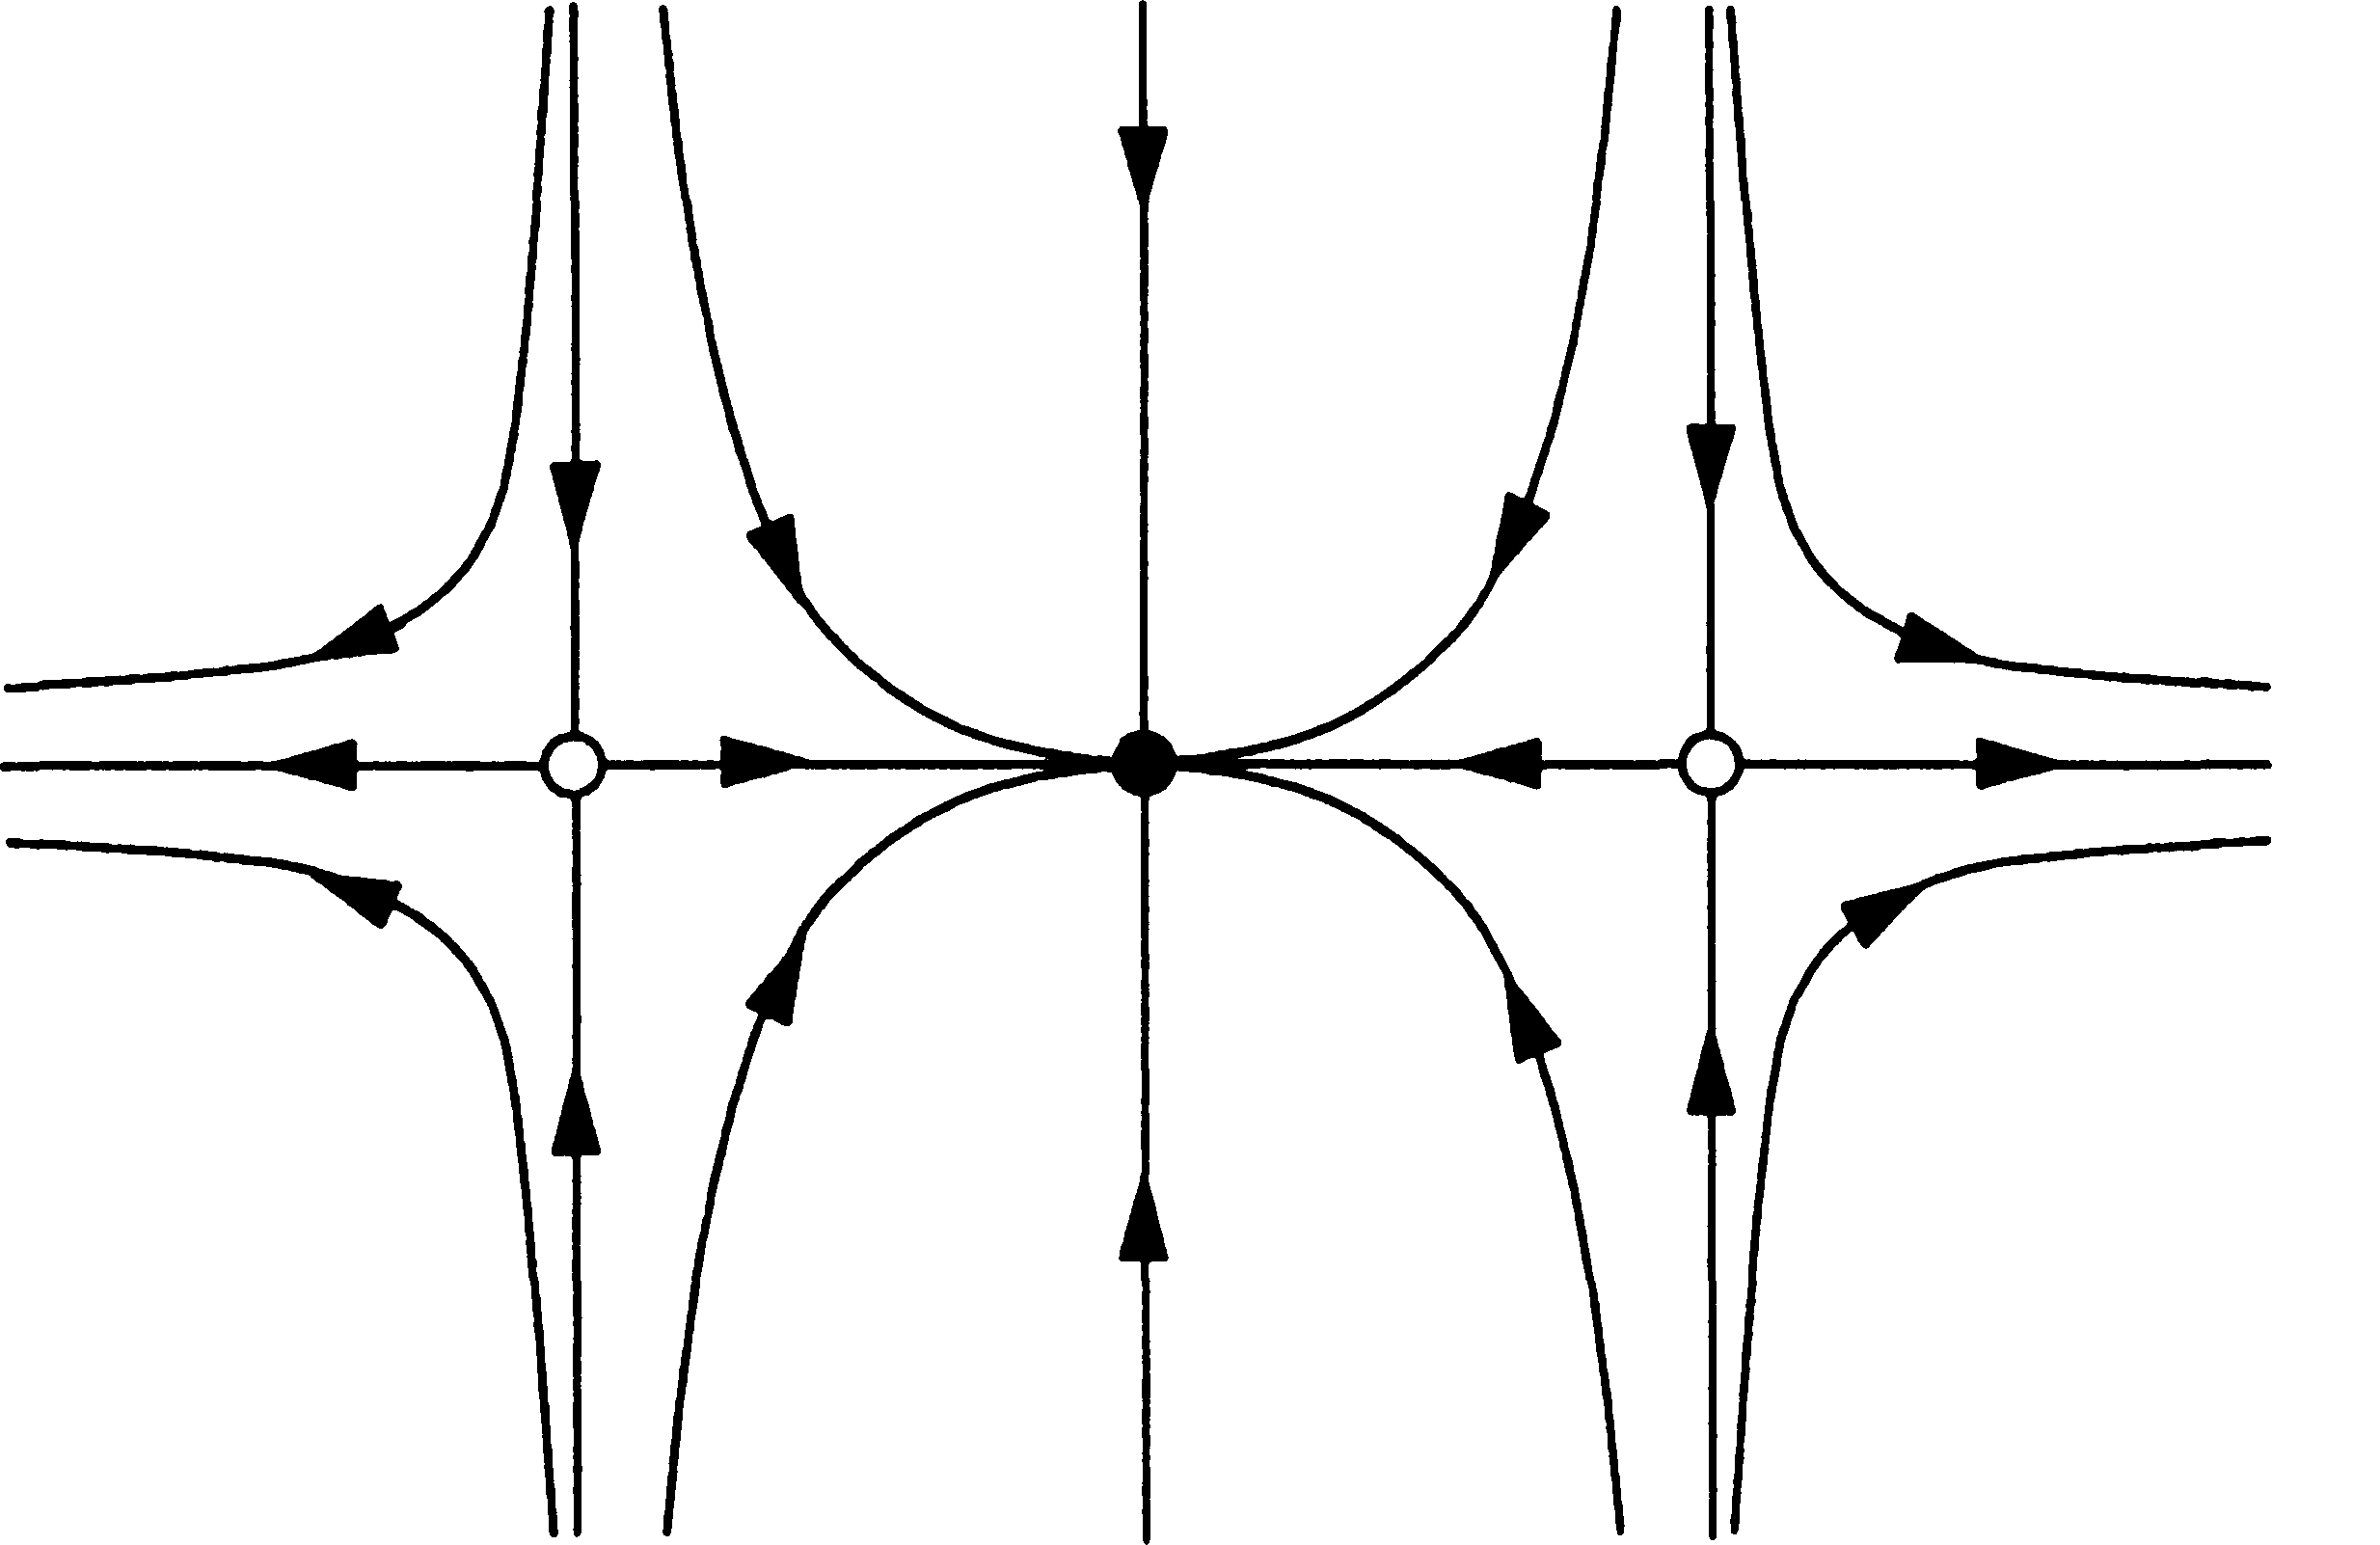
\includegraphics[width=0.82\textwidth]{images/Figures/figur-007.png}
\caption{Örnek 6.3.1 için doğrusal olmayan sistemin faz portresi.}
\label{fig:6-3-1}
\end{figure}

Bu resim, lineerleştirmeden beklendiği gibi $(0,0)$ noktasının kararlı düğüm, $(\pm1,0)$ noktalarının ise eyer olduğunu doğrular.
\end{justify}

\subsection*{Örnek 6.3.2}
\phantomsection
\addcontentsline{toc}{subsection}{Örnek 6.3.2}

\begin{justify}
Aşağıdaki sistemi ele alalım:
\begin{align}
\dot{x} &= -y+a x(x^2+y^2),\\
\dot{y} &= x+a y(x^2+y^2),
\end{align}
burada $a$ bir parametredir. Lineerleştirilmiş sistemin orijinin tüm $a$ değerleri için merkez olduğunu yanlış biçimde öngördüğünü; oysa gerçekte $a<0$ için orijinin kararlı spiral, $a>0$ için ise kararsız spiral olduğunu gösterin.

\textbf{Çözüm.} $(x^{*},y^{*})=(0,0)$ etrafındaki lineerleştirmeyi elde etmek için Jacobian matrisini doğrudan tanımdan hesaplayabiliriz. Ya da şu kısa yolu kullanabiliriz: Orijinde sabit noktası olan herhangi bir sistemde $x$ ve $y$, sabit noktadan sapmaları temsil eder; çünkü $u=x-x^{*}=x$ ve $v=y-y^{*}=y$ olur. Bu nedenle $x$ ve $y$ cinsinden doğrusal olmayan terimleri atarak lineerleştirme yapılabilir. Böylece lineerleştirilmiş sistem
\begin{align}
\dot{x} &= -y,\\
\dot{y} &= x
\end{align}
olur. Jacobian matrisi
\begin{equation}
A=\begin{pmatrix}0&-1\\1&0\end{pmatrix}
\end{equation}
şeklindedir. Bu matris için iz $\tau=0$ ve determinant $\Delta=1>0$ olduğundan lineerleştirmeye göre orijin her zaman bir merkezdir.

Doğrusal olmayan sistemi analiz etmek için kutupsal koordinatlara geçelim. $x=r\cos\theta$ ve $y=r\sin\theta$ olsun. $r$ için bir diferansiyel denklem türetmek amacıyla $x^2+y^2=r^2$ olduğuna dikkat edelim. Buradan
\begin{equation}
x\dot{x}+y\dot{y}=r\dot{r}
\end{equation}
elde edilir. $\dot{x}$ ve $\dot{y}$ yerine yazılırsa
\begin{align}
r\dot{r} &= x[-y+a x(x^2+y^2)]+y[x+a y(x^2+y^2)]\\
&= a(x^2+y^2)^2\\
&= ar^4
\end{align}
bulunur. Dolayısıyla
\begin{equation}
\dot{r}=ar^3.
\end{equation}
Alıştırma 6.3.12'de, $\theta$ için aşağıdaki diferansiyel denklemi türetmeniz istenir:
\begin{equation}
\dot{\theta}=\frac{x\dot{y}-y\dot{x}}{r^2}.
\end{equation}
$\dot{x}$ ve $\dot{y}$ yerine yazıldığında $\dot{\theta}=1$ bulunur. Böylece özgün sistem kutupsal koordinatlarda
\begin{align}
\dot{r} &= ar^3,\\
\dot{\theta} &= 1
\end{align}
biçimine dönüşür.

Bu biçimde sistemi analiz etmek kolaydır; çünkü radyal ve açısal hareketler birbirinden bağımsızdır. Tüm yörüngeler orijin etrafında sabit açısal hız $\dot{\theta}=1$ ile döner.

Radyal hareket $a$ değerine bağlıdır ve Şekil~\ref{fig:6-3-2}'de gösterilecektir. Eğer $a<0$ ise $t\to\infty$ iken $r(t)$ monoton olarak $0$'a gider. Bu durumda orijin kararlı spiraldir. Ancak sönüm çok yavaştır; bu durum bilgisayar tarafından üretilen yörüngelerde de görülebilir. Eğer $a=0$ ise tüm $t$ değerleri için $r(t)=r_0$ olur ve orijin merkezdir. Son olarak $a>0$ ise $r(t)$ monoton olarak sonsuza gider ve orijin kararsız spiraldir.

\begin{figure}[H]
\centering
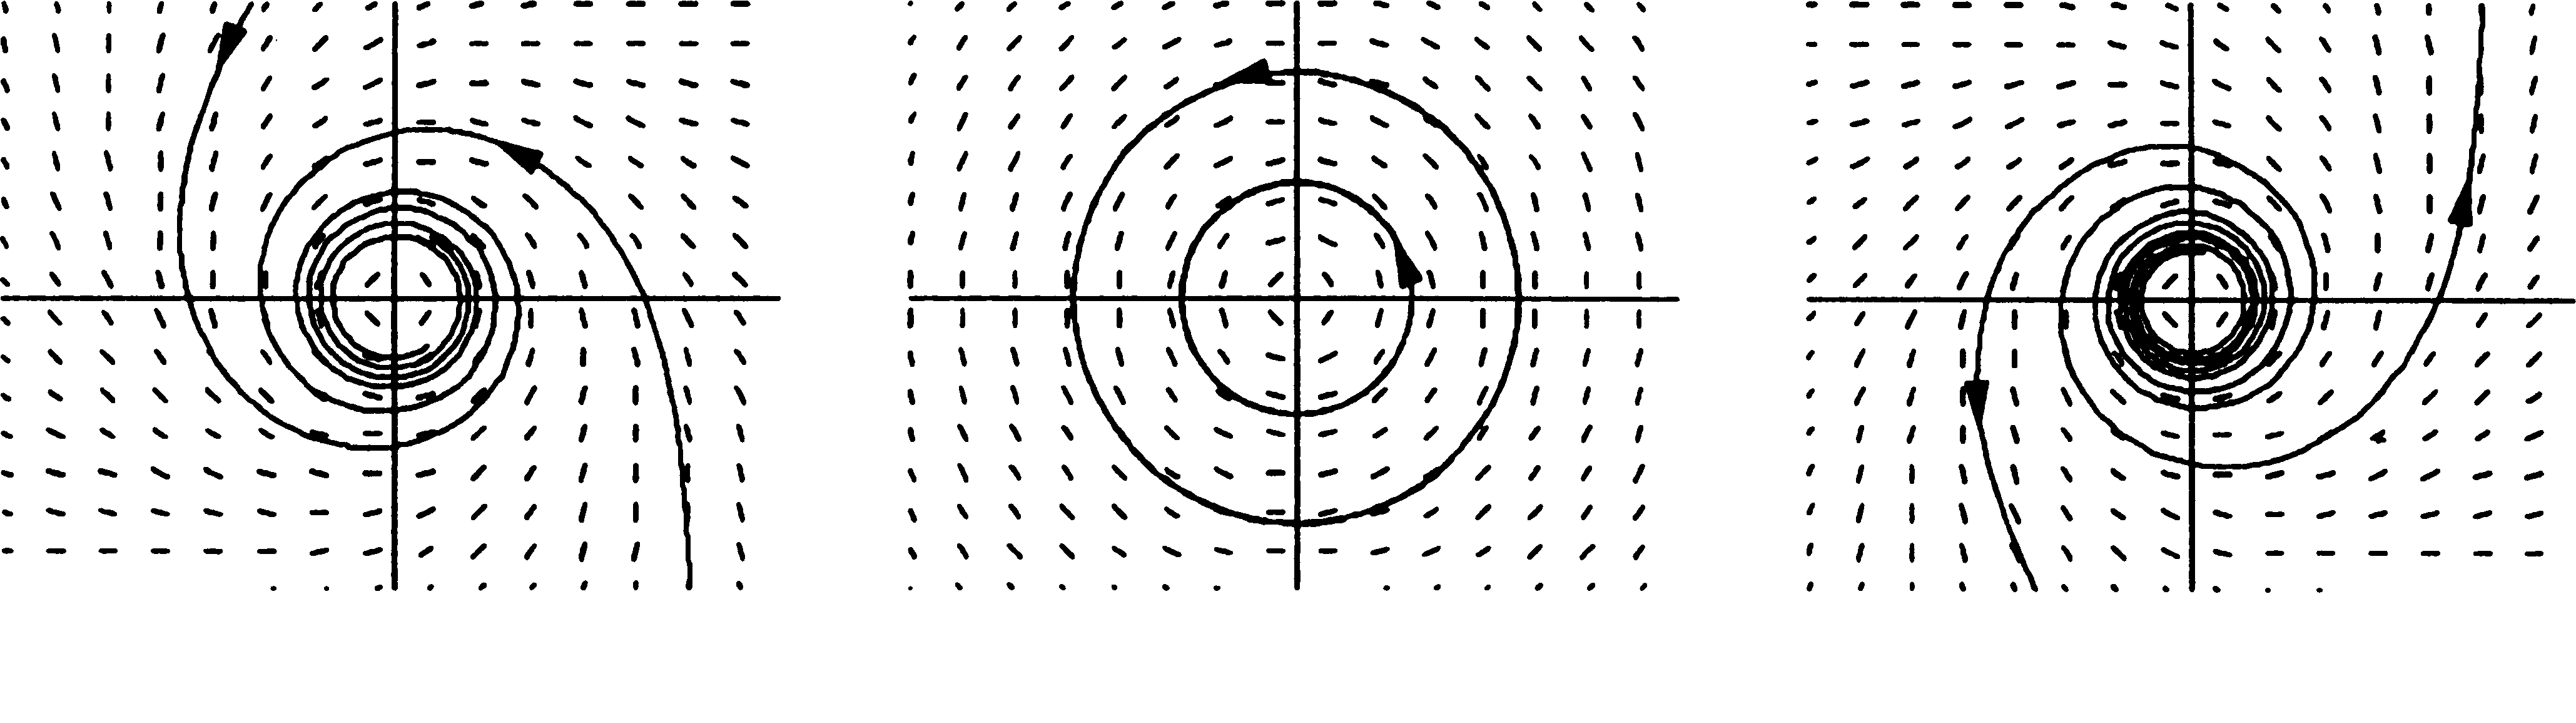
\includegraphics[width=0.82\textwidth]{images/Figures/figur-008.png}
\caption{Parametre değerlerine göre orijin yakınındaki davranış: $a<0$, $a=0$ ve $a>0$.}
\label{fig:6-3-2}
\end{figure}

Artık merkezlerin neden bu kadar hassas olduğunu görebiliriz: Tüm yörüngelerin bir çevrimden sonra kusursuz biçimde kapanması gerekir. En küçük bir sapma merkezi spirale dönüştürür.
\end{justify}

\subsection*{Hiperbolik Sabit Noktalar, Topolojik Eşdeğerlik ve Yapısal Kararlılık}
\phantomsection
\addcontentsline{toc}{subsection}{Hiperbolik Sabit Noktalar, Topolojik Eşdeğerlik ve Yapısal Kararlılık}

\begin{justify}
Benzer biçimde, yıldızlar ve yozlaşmış düğümler de küçük doğrusal olmayan etkilerle değiştirilebilir; fakat merkezlerden farklı olarak bunların kararlılığı değişmez. Örneğin kararlı bir yıldız, kararlı bir spirale dönüşebilir; fakat kararsız bir spirale dönüşmez. Bu durum, doğrusal sistemlerin sınıflandırılması düşünüldüğünde makuldür: yıldızlar ve yozlaşmış düğümler kararlı ya da kararsız bölgenin içinde yer alırken, merkezler kararlılık ile kararsızlık arasındaki hassas sınırda bulunur.

Eğer yörüngelerin ayrıntılı geometrisiyle değil yalnızca kararlılıkla ilgileniyorsak, sabit noktaları daha kaba biçimde şöyle sınıflandırabiliriz:

\textbf{Sağlam durumlar:}
\begin{itemize}
\item \textbf{İticiler} ya da \textbf{kaynaklar}: Her iki özdeğerin reel kısmı pozitiftir.
\item \textbf{Çekiciler} ya da \textbf{yutaklar}: Her iki özdeğerin reel kısmı negatiftir.
\item \textbf{Eyerler}: Özdeğerlerden biri pozitif, diğeri negatiftir.
\end{itemize}

\textbf{Marjinal durumlar:}
\begin{itemize}
\item \textbf{Merkezler}: Her iki özdeğer saf sanaldır.
\item \textbf{Daha yüksek mertebeden ve izole olmayan sabit noktalar}: En az bir özdeğer sıfırdır.
\end{itemize}

Dolayısıyla kararlılık açısından marjinal durumlar, en az bir özdeğerin $\operatorname{Re}(\lambda)=0$ koşulunu sağladığı durumlardır.

Her iki özdeğer için $\operatorname{Re}(\lambda)\neq0$ ise sabit nokta genellikle \textbf{hiperbolik} olarak adlandırılır. Bu ad biraz talihsizdir; çünkü kulağa yalnızca eyer noktası anlamına geliyormuş gibi gelir, ancak standart terim hâline gelmiştir. Hiperbolik sabit noktalar dayanıklıdır; kararlılık türleri küçük doğrusal olmayan terimlerden etkilenmez. Hiperbolik olmayan sabit noktalar ise hassas olanlardır.

Doğru üzerindeki vektör alanları bağlamında hiperbolikliğin basit bir örneğini daha önce gördük. Bölüm 2.4'te, $f'(x^{*})\neq0$ olduğu sürece sabit noktanın kararlılığının lineerleştirme tarafından doğru biçimde öngörüldüğünü gördük. Bu koşul, $\operatorname{Re}(\lambda)\neq0$ koşulunun tam karşılığıdır.

Bu fikirler daha yüksek mertebeden sistemlere de düzgün biçimde genellenir. $n$ mertebeli bir sistemin sabit noktası, lineerleştirmenin tüm özdeğerleri sanal eksen dışında yer alıyorsa hiperboliktir; yani $i=1,\ldots,n$ için $\operatorname{Re}(\lambda_i)\neq0$ olmalıdır. Önemli Hartman--Grobman teoremi, hiperbolik bir sabit nokta yakınındaki yerel faz portresinin lineerleştirmenin faz portresiyle \textit{topolojik olarak eşdeğer} olduğunu söyler. Özellikle, sabit noktanın kararlılık türü lineerleştirme tarafından doğru biçimde yakalanır.

Burada topolojik eşdeğerlik, bir yerel faz portresini diğerine taşıyan bir homeomorfizmanın, yani sürekli tersi olan sürekli bir deformasyonun bulunması anlamına gelir. Bu dönüşüm yörüngeleri yörüngelere götürür ve zaman yönünü, yani okların yönünü korur.

Sezgisel olarak iki faz portresi, biri diğerinin bozulmuş bir biçimiyse topolojik olarak eşdeğerdir. Eğme ve bükmeye izin vardır; fakat yırtmaya izin yoktur. Dolayısıyla kapalı yörüngeler kapalı kalmalı, eyer noktalarını birleştiren yörüngeler kopmamalıdır.

Hiperbolik sabit noktalar ayrıca yapısal kararlılık denen önemli genel kavramı da gösterir. Bir faz portresi, vektör alanına yapılan keyfî derecede küçük bir bozunumla topolojisi değiştirilemiyorsa yapısal olarak kararlıdır. Örneğin bir eyer noktasının faz portresi yapısal olarak kararlıdır; ancak bir merkezin faz portresi değildir. Çünkü keyfî derecede küçük bir sönüm, merkezi spirale dönüştürür.
\end{justify}


\newpage
